%TODO Remove relations to ParMA, this paper should be more focused on the simultations and results that we get as well as the constructions for each application and the nuaisses that EnGPar can represent.

\section{Introduction}


\section{Notation}
\begin{itemize}
  \item $M^d$ a set of mesh entities of dimension $d$.
  \item $M_i^d$ the $i$th mesh entity of dimension $d$.
  \item $V$ a set of vertices $u_i$ which uniquely
    exist on one part such that $V = \bigcup_{\forall_i}u_i$.
  \item $E_i$ a set of relations $e_{ij}$ of type $i$ that represent a
    edge between two vertices, $u,v\in V$ such that $E_i = \bigcup_{\forall_j}e_{ij}$.
  \item $H_i$ a set of relations $h_{ij}$ of type $i$ that represent a
    hyperedge between a set of vertices such that $H_i = \bigcup_{\forall_j}h_{ij}$.
  \item $V_{h_{ij}}$ the set of vertices the hyperedge $h_{ij}\in H_i$ connects.
  \item $P_i$ a set of pins which represent the connection from hyperedge
        $h_{ij}$ to $v$ where $h_{ij} \in H_i$ and $v \in V_{h_{ij}}$.
\end{itemize}

\section{Partitioning}

\subsection{(Hyper)Graph partitioners}
Graph-based partitioning methods are a common way to perform
load balancing on relational data. These methods require
the data to be transformed into a graph structure. The idea of this
construction is such that the vertices represent a unit of work
and the relations between the work form the edges of the graph.
When this graph is partitioned the vertices are uniquely divided
between the parts and the edges that cross the part boundaries
represent communication between the connected parts. Graph
partitioners split the graph into $k$ parts 
where each part has the same amount of work and the inter part
communication is minimized. Parallel multi-level techniques
applied to graphs have been shown to produce high-quality
partitions up to tens of thousands of parts quickly and efficiently
\cite{catalyurek2013umpa,karypis1999parallel,lasalle2013multi,schloegel2002parallel}.

Hypergraph methods improve graph partitioning methods, using
hyperedges to better represent more complex forms of
communication. These hyperedges allow relations
between multiple sets of work or graph vertices. In
many cases, including unstructured meshes and sparse matrices,
hypergraph partitioning has been shown to reduce the
communication costs of the final partition
\cite{catalyurek1999hypergraph,catalyurek2009repartitioning,devine2006parallel}.
While these methods produce better partitions of the data,
they are more computational and memory intensive relative
to graph-based methods.

\subsection{Geometric methods}
%RIB/RCB

\subsection{Diffusive partitioning}
Diffusive partitioning techniques perform improvements to existing
partitions by migrating load across part boundaries. These migrations
are either controlled globally, or locally computed on each part.
The global methods select weight to migrate in order to minimize
the total weight transferred or the maximum weight transferred
in or out of a part \cite{hu1999improved,ou1994parallel}. Local
diffusive partitioners transfer load iteratively from parts
with more work to neighboring parts with less
\cite{cybenko1989dynamic,subramanian1994analysis}. This approach
combined with heuristics for how the load is transferred can have
significantly less computational cost than global methods
\cite{Fiduccia1982,Kernighan1970}. 

\section{N-graph}
EnGPar interfaces to the different partitioning procedures through a multigraph
abstraction called the N-graph. A multigraph
\cite{BANGJENSENmultigraph, BOESCHmultigraph} is a graph that supports multiple
edges between two vertices. Towards
supporting a combination of (hyper)graph, geometric, and diffusive partitioning
methods on relation-based data, the N-graph is defined using one of two modes.
The first is a traditional multigraph with a set of vertices $V$ and $n$
different sets of edges $E_0,...,E_{n-1}$. The N-graph also supports a
multi-hypergraph mode utilizing hyperedges to better represent certain types
of relations. This mode is defined by a set of vertices $V$, $n$ sets of
hyperedges $H_0,...H_{n-1}$ and $n$ sets of pins $P_0,...,P_{n-1}$ which
connect the vertices and hyperedges.

The hyperedge mode for the
N-graph is well suited to relate vertices that share a single connection
between greater than two vertices. Take for instance the construction of
an N-graph given an
unstructured mesh. Mesh elements, $M^3$, are represented
by graph vertices and mesh vertices, $M^0$, are used for
relations between mesh elements. Depending on the mode, edges/hyperedges and
pins will be added to represent these relations. In the
traditional graph mode, an edge is created between two
graph vertices if the mesh elements they represent share a mesh
vertex. In the hypergraph mode, one hyperedge is made for
each mesh vertex. Also, a pin is created to connect a
graph vertex and graph hyperedge if the corresponding mesh
element is bounded by the mesh vertex. To examine these two modes, let
$n$ be the number of mesh elements that bound a certain mesh vertex. On average
in a three-dimensional tetrahedron mesh, $n$ is 23 \cite{beall1997general}. To
represent this relation between all $n$ graph vertices in the N-graph with
traditional edges would require $O(n^2)$ edges in the N-graph. However, when
using hyperedges one
graph edge is created to represent the mesh vertex and $O(n)$ pins to connect
the graph vertices and hyperedges. This results in a reduction in memory usage.
%[TODO].
%as well as runtime improvements for certain graph operations.
Figure \ref{fig:edgecounts} gives an example 2D mesh
where seven mesh elements bound a mesh vertex (a). The
N-graph of this mesh constructed using mesh faces
as graph vertices and vertices for faces is shown in
(b) using traditional edges and in (c) with hyperedges.
In (b) fifteen graph edges are created for the one mesh
vertex while in (c) one hyperedge is added and seven
pins connect the graph vertices to the hyperedge.

\begin{figure}[!ht]
  \centering
  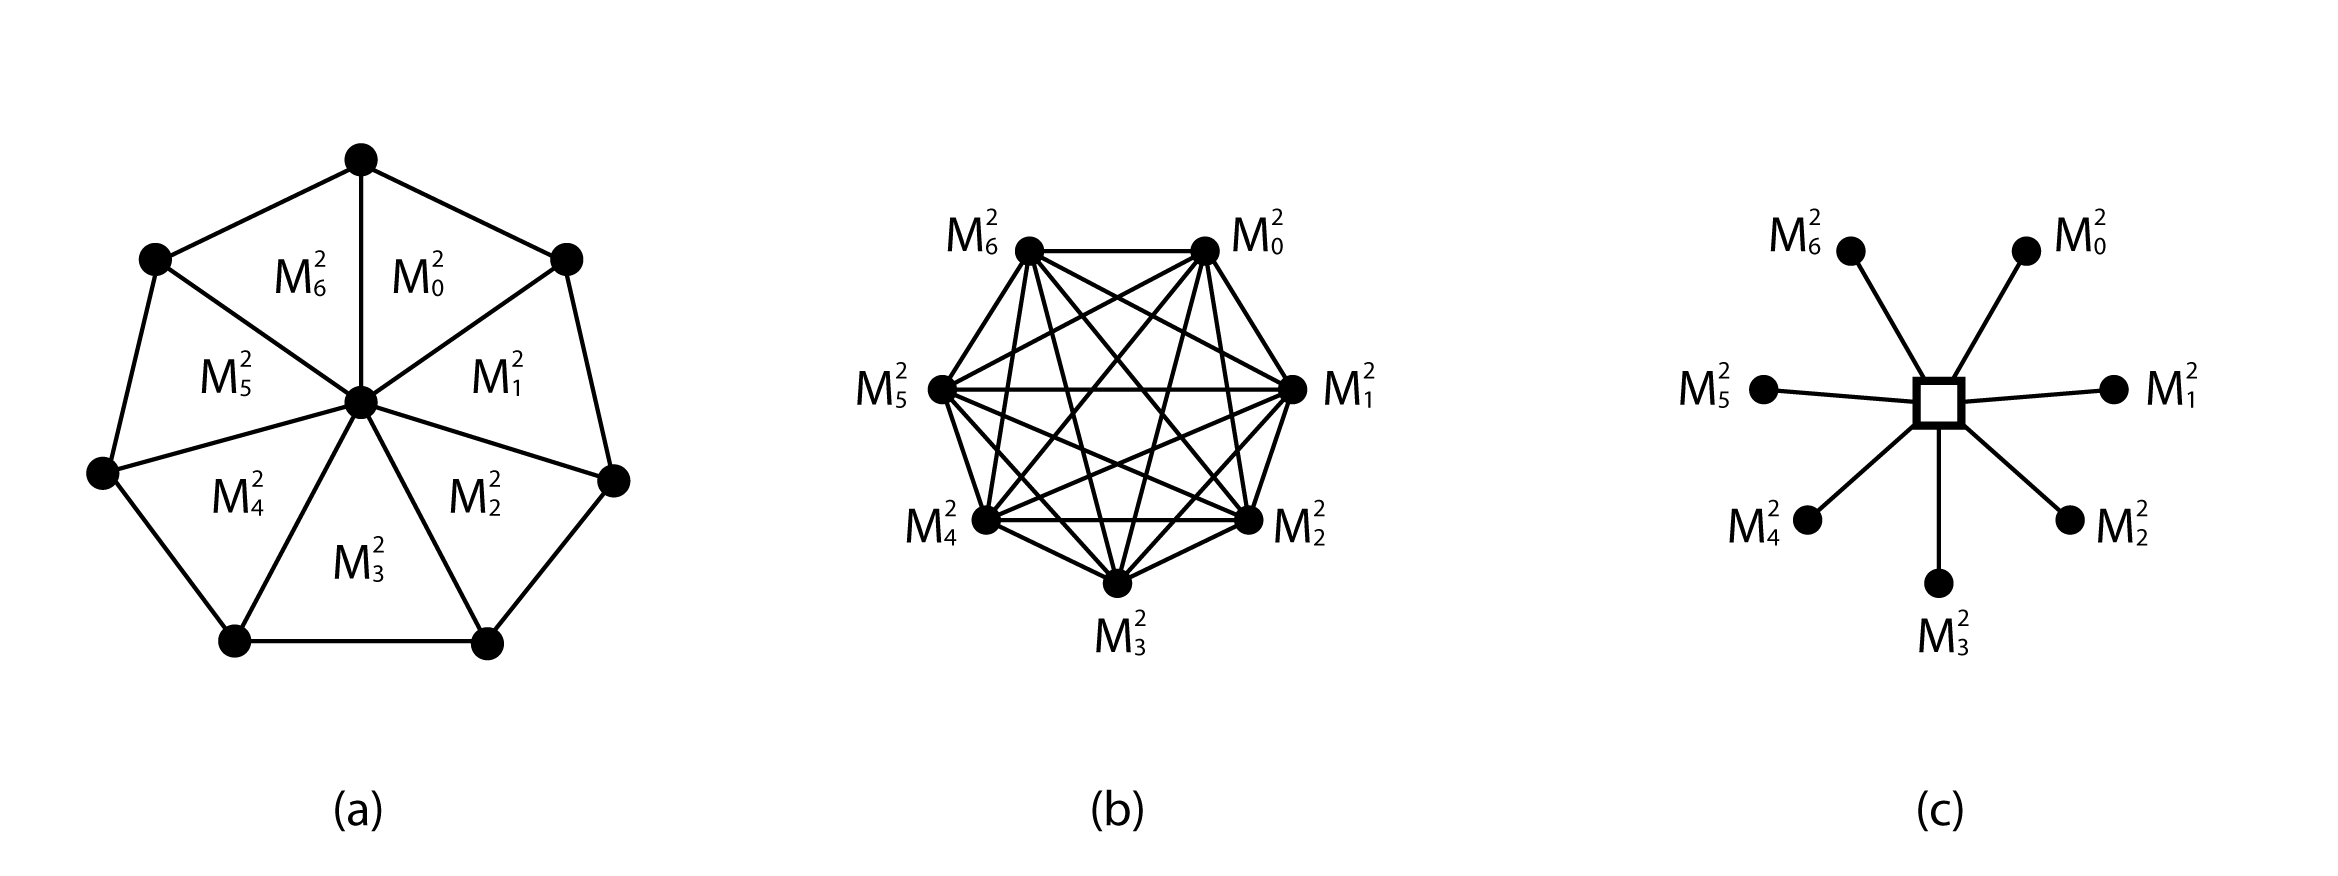
\includegraphics[width=3.5in]{../figures/edgecounts.png}
  \caption{(a) a seven triangle mesh surrounding one vertex. (b) N-graph constructed around the vertex using traditional edges to connect the graph vertices whose corresponding mesh elements share the mesh vertex. (c) The N-graph construction using a hyperedge for the mesh vertex and connecting the adjacent mesh elements with pins in the N-graph.}
  \label{fig:edgecounts}
\end{figure}

The N-graph also supports having multiple edge types,
whether using traditional edges or hyperedges. This
allows representing multiple layers of connection
between the graph vertices. This is useful to represent
applications that use multidimensional data or complex
levels of communication. One example is an unstructured
mesh which have vertices,
edges, and faces (in three dimensions) that are shared
between mesh elements. To represent these data
structures for a range of application needs, the
N-graph supports the arbitrary use of edge types to allow
different configurations for applications. Figure
\ref{fig:Mesh2Graph} depicts the mapping of a 2D unstructured mesh (a) to a
representation where mesh elements map to graph vertices and mesh vertices map
to graph hyperedges (b). In (c) a second mapping is shown where mesh edges
are also mapped to a second edge type in the graph. The labels of the entities
in (a) are carried to (b) and (c) to show which mesh entity is represented by
the corresponding graph entity.

\begin{figure}[!ht]
  \centering
  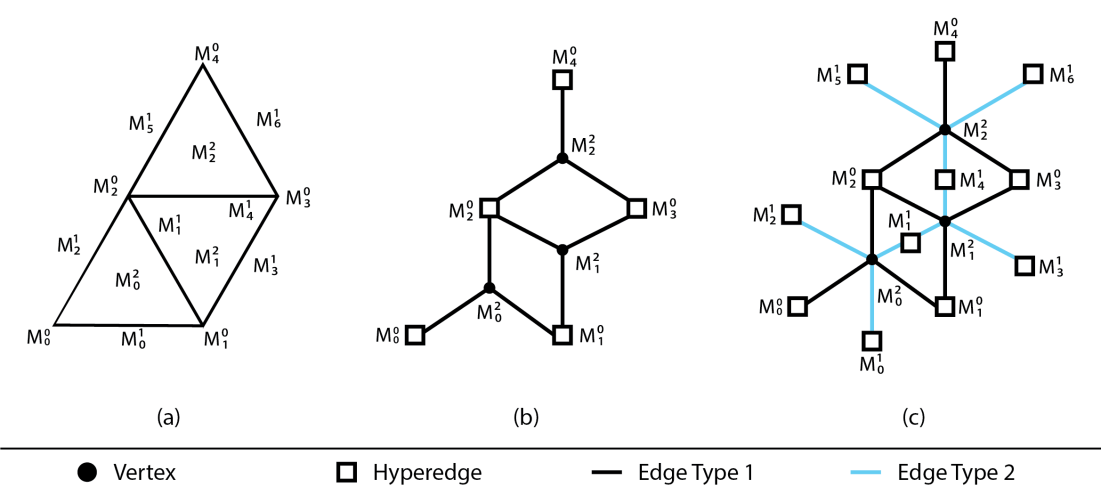
\includegraphics[width=3.5in]{../figures/exampleMesh2Graph.png}
  \caption{(a) a 2D unstructured mesh. (b) N-graph construction with elements$\rightarrow$vertices, vertices$\rightarrow$hyperedges. (c) additional mesh edges are used for a second set of hyperedges. Mesh labeling is shared in all three to correlate mesh entities to graph entities.}
  \label{fig:Mesh2Graph}
\end{figure}


%TODO minimize this section to include only the important parts of the algorithm. Add information on anything that sepcifically aids the applications in this paper.
\section{Diffusive Load Balancing}
%What is the algorithm? Summarize the stuff that is the same as ParMA.  Focus on
%the differences and improvements.
The diffusive load balancing techniques used in both ParMA and EnGPar follow
the same basic framework. The techniques iteratively perform a series of steps
until user specified criteria are met or the algorithm can not improve
the partition quality further. The main metric used in EnGPar for partition quality is the imbalance of a set of entities. This value is defined by calculating the sum of the weights of the entities in each part. Then, the maximum across all parts is divided by the average. For example, when equal weights are used, the imbalance of vertices in the N-graph is the maximum number of vertices on a single part divided by the average number of vertices per part, across all processes.

Algorithm \ref{alg:engpar} lists a general
framework of the multi-criteria load balancing procedures in ParMA.

\begin{algorithm}
\caption{ParMA Load Balancing Framework}
\label{alg:engpar}
\small
\begin{algorithmic}[1]
  \Procedure{RunStep}{$mesh$,$d$}
    \State -Determine the neighboring parts and size of part boundaries.
    \State -Compute the weight of the entities in dimension $d$
    \State -Share the computed weight with each neighbor.
    \State -Determine which neighbors that can receive more weight.
    \State -Calculate how much weight to send to each neighbor.
    \State -Construct an ordering of vertices to traverse the part boundary.
    \State -Create migration plan that reduces the imbalance of dimension $d$.
    \State -Adjust the plan to maintain balance of previous dimensions.
    \State -Perform Migration
  \EndProcedure
  \Procedure{Balance}{$mesh$,$dimensions$}
    \ForAll{$d \in dimensions$}
      \While{imbalance of $d$ > tolerance}
        \Call{RunStep}{$mesh$,$d$}
        \If{Balancing Stagnates}
          \State break
        \EndIf
      \EndWhile
    \EndFor
  \EndProcedure
\end{algorithmic}
\end{algorithm}

The framework's \texttt{BALANCE} procedure iteratively
calls \texttt{RUNSTEP} to improve the
target imbalance. The \texttt{RUNSTEP} procedure performs six
stages to determine the diffusive load balancing of each
step. The first step on line 2 determines who are the
neighbors of each part and what is the size of the part
boundaries between them. The second computes the weight
of the target dimension $d$ and sends the weight to the
neighboring parts on lines 3 and 4. Then, the heavy
parts decide which neighbors to send weight to and how
much to send on lines 5 and 6. The fourth stage constructs
an ordering of the entities on the boundary for selecting
on line 7. Lines 8 and 9 select entities to be migrated
to the neighboring parts. Finally, a migration is performed
to send the selected entities to neighboring parts on line 10.

The input to the \texttt{BALANCE}
procedure, $dimensions$, is an ordering of the criteria
to be balanced. It is interpreted such that earlier
entries have higher priorities and thus will be balanced
first and their reduced imbalance will be maintained in following
steps. Line 8
of Algorithm \ref{alg:engpar} adjusts the migration plan to
ensure that the imbalance of completed dimensions is not
increased. An example of multi-criteria load balancing
is the ``vertex > element'' case for finite element
methods when degrees of freedom are defined by the mesh vertices.
The degrees of freedom contain the largest
portion of computational work in these simulations
and thus, make balancing the mesh vertices a top
priority. However, these simulations also require balancing
the mesh elements for efficient linear system assembly.
In this example mesh vertices would be the first criteria
followed up by mesh elements.

The work to improve the multi-criteria load
balancing in EnGPar is focused
on two aspects of this algorithm. One is the
generalization to support for a larger range of applications
while the second is to improve the speed of the
more communication and computational expensive parts.
Each of these is discussed in more detail in the following sections.

\subsection{Generalization of Multicriteria Load Balancing}
The generalization of the framework in EnGPar to support more
applications is partially completed with the usage of the N-graph.
Since ParMA works directly on meshes, it cannot 
scale-free graphs \cite{pienta2013parallel,gonzalez2012powergraph}
or directly work with unstructured
meshes using vertex-based partitions. Since EnGPar utilizes
the N-graph, it natively
supports other relation based data.

Beyond supporting other forms of data, many applications have
different priorities of balancing the different criteria. While
ParMA is built to perform load balancing targeting finite element
applications, EnGPar takes a more general approach
allowing users to define the ordering and tolerances of criteria.
This is highlighted in Algorithm \ref{alg:engpar} on line 11 with
the $dimensions$ argument. This argument controls the ordering in
which dimensions are balanced with earlier dimensions having higher
priority. In ParMA these inputs would be defined by the balancer
that is applied. Meaning that for ParMA to support additional
applications new balancers need to be defined for the user to use.
In EnGPar the users can use any ordering of priorities
without any new development. This is done by providing
a richer user interface with inputs to control all
necessary components of the diffusive balancing procedure.

\subsection{Graph Distance}
One of the optimizations in ParMA targets decreasing surface area across parts
by ordering the selection of elements to migrate based on their topological
distance from the center of the part. Several challenges arise in the method
due to the existence of disconnected components throughout the part. To get
an optimal ordering it is important to offset the distances of the disconnected
components such that shallower components get a higher priority. This leads to
the shallower components being migrated first. 

ParMA computes the graph distance using multiple breadth-first traversals; one
traversal to find disjoint sets, another to locate the topological centers of
each set, and another to compute the distance.
EnGPar reduces the number of traversals from three to two. This
is done by locating the disconnected components during the
traversal to compute distances using a disjoint set data structure.

EnGPar's distance computation algorithm is listed in
Algorithm~\ref{alg:graphdist}. The general breadth-first
traversal is on lines 1 to 5. This performs a
traversal over the entire graph where every time a vertex
is reached the input $kernel$ is run. The algorithm begins
by calling \texttt{COMPUTEDISTANCE}. On line 51, the initial
traversal is used to find the topological center of all
disconnected components simultaneously as well as
the depth of each vertex. The first traversal is seeded
by the vertices that are on the part boundary. Then, an
additional traversal is performed on lines 55-60. This traversal is seeded
by the deepest vertices of the first traversal found
in the \texttt{SETLABELS} procedure on lines 25-39. This
traversal is repeated until every vertex has a
distance by computing the next deepest level of vertices
that does not have a distance.

When multiple vertices share the same depth,
it is possible that multiple disconnected components will
be traversed simultaneously. To differentiate the
components, a disjoint set  is initialized for each
vertex in the deepest level. The disjoint set data
structure, commonly known for its use in Kruskal's
algorithm for finding minimum spanning trees \cite{disjointset}, allows fast joining
and comparison of sets. The data structure consists of a label for each vertex
and a parent pointer that initially points to itself. When two sets are unioned,
one of the sets is chosen as the parent and the other set points its parent
pointer to that set. This allows all sets to be represented by its highest
parent allowing comparison of two sets in $O(\log{n})$, in the average case,
where $n$ is the number of sets in the beginning. The
remaining usage of the disjoint sets
is in the \texttt{DISTANCE\_KERNEL} on lines 15-19 where new vertices are assigned
a label and already assigned vertices are unioned together. If there are
multiple disjoint sets after the traversal is complete,
the distances of each disjoint
set is offset such that the deepest disjoint sets have lower distances.

\begin{algorithm}
  \caption{EnGPar Graph Distance Computation}\label{alg:graphdist}
  \small
  \begin{algorithmic}[1]
    \Procedure{Traversal}{$seed$, $graph$, $kernel$}
      \State Breadth-first traversal of the $graph$ vertices
      \State starting with the $seed$ vertices.
      \State The $kernel$ is called for each visited vertex.
    \EndProcedure
    \Procedure{depth\_kernel}{$u$, $G$}
      \For{ $v \in e(u,v)$ }
         \If{ not $visited(v)$ }
            \State $depth(v) \gets depth(u)+1$
         \EndIf
      \EndFor
    \EndProcedure
    \Procedure{distance\_kernel}{$u$, $G$}
      \For{ $v \in e(u,v)$ }
         \If{ not \Call{find}{$v$} }
           \State $label(v) \gets$ \Call{find}{$u$}
         \ElsIf{ \Call{find}{$u$} != \Call{find}{$v$} }
           \State \Call{union}{$u$,$v$}
           \Comment{{\tiny merge them into the same set}}
         \EndIf
         \If{ not $visited(v)$ }
            \State $distance(v) \gets distance(u)+1$
         \EndIf
      \EndFor
    \EndProcedure
    \Procedure{setLabels}{$visited$,$levels$}
      \State $init \gets \emptyset$
      \For{ $u \in levels$ }
        \If{ not $visited(u)$ }
          \State break
        \EndIf
      \EndFor
      \State $maxdepth \gets depth(u)$
      \For{ $u \in levels$ }
        \If{ not $visited(u)$ and $depth(u) == maxdepth$ }
           \State $init \gets init \bigcup u$
        \EndIf
      \EndFor
      \State \textbf{return} $init$
    \EndProcedure
    \Procedure{maxVisitedDepth}{$visited$}
      \State $depth \gets 0$
      \For{ $u \in visited$ }
        \If{ $visited(u)$ and $depth < depth(u)$}
          \State $depth \gets depth(u)$
        \EndIf
      \EndFor
      \State \textbf{return} $depth$
    \EndProcedure
    \Procedure{computeDistance}{$G$}
      \State $init \gets$ vertices classified on ${d-1}$ partition model entities
      \State \Call{Traversal}{$init$,$G$,$depth\_kernel$}
      \State $levels \gets$ \Call{sort}{$G$}
      \Comment{{\tiny $levels$ is an array vertices in order of decreasing depth}}
      \State $visited \gets array(|V|,0)$
      \State $depth \gets 0$
      \While{ $init \gets$ \Call{setlabels}{$visited$,$levels$} }
        \Comment{{\tiny Label the vertices with the largest remaining
                 depth.  If none remain, then break from the while loop.}}
        \State foreach $u \in init$: \Call{makeSet}{$u$}
        \State foreach $u \in init$: $depth(u) \gets depth$
        \State \Call{Traversal}{$init$,$G$,$distance\_kernel$} \label{step:distbfs}
        \State $depth \gets$ \Call{maxVisitedDepth}{$visited$}
      \EndWhile
    \EndProcedure
  \end{algorithmic}
\end{algorithm}

%see
%\url{http://www.csl.mtu.edu/cs4321/www/Lectures/Lecture\%2019\%20-\%20Kruskal\%20Algorithm\%20and\%20Dis-joint\%20Sets.htm}
%for details of Kruskal's disjoint set procedures

%These sections should include the construction for the application as well as experiments and results
\section{Unstructured Mesh Applications}

\subsection{Phasta}

\subsection{FUN3D}

\subsection{XGC: Particle In Cell}


\section{Closing Remarks and Future Work}

\begin{acks}
This research is supported by the National Science
Foundation under Grant ACI 1533581. The support of
the U.S. Department of Energy, Office of Science,
Office of Advanced Scientific Computing Research,
under award DE-SC00066117 (FASTMath SciDAC Institute)
is also acknowledged.

An award of computer time was provided by the Innovative and Novel
Computational Impact on Theory and Experiment (INCITE) program and a separate
award of computer time by the Theta Early Science program.
This research used resources of the Argonne Leadership Computing Facility,
which is a DOE Office of Science User Facility supported under Contract
DE-AC02-06CH11357.
\end{acks}
